\section{Metrics}
\label{sec:metrics}
We use several metrics (in SI units) to evaluate and compare the performance of RMA against baselines:
\begin{itemize}
    \item Success Rate: Average rate of successfully completing the task as defined in the next section. 
    \item Time to Fall (TTF): Measures the time before a fall. We divide it by the maximum duration of the episode and report a normalized value between $0$ and $1$.
    \item Reward: Average step forward reward plus lateral reward over multiple episodes as defined in Section III-A RL Rewards of the main paper. 
    \item Distance: Average distance covered in an episode. For real-world experiments, we report the normalized distance, where we normalize by the maximum distance which is specific to the task.
    \item Adaptation Samples: Number of control steps to explore in the testing environment needed for the motor policy to adapt.
    \item Torque: Squared L2 norm of torques at every joint $\| \bm{\tau}^{t} \|^2$.
    \item Jerk: Squared L2 norm of delta torques $\| \bm{\tau}^{t} - \bm{\tau}^{t-1} \|^2$.
    \item Ground Impact: Squared L2 norm of delta ground reaction forces at every foot $\|\mathbf{f}^t - \mathbf{f}^{t-1}\|^2$. 
\end{itemize}



\section{Additional Training and Deployment Details}
The training pipeline is shown in Algorithm \ref{algo:training}, and the deployment pipeline is shown in Algorithm \ref{algo:deployment}.

We use PPO \cite{schulman2017proximal} to train the base policy and the environmental factor encoder. We train for total $15,000$ iterations. During each iteration, we collect a batch of $80,000$ state-action transitions, which is evenly divided into $4$ mini-batches. Each mini-batch is fed into the base policy and the Environment Factor Encoder in sequence for 4 rounds to compute the loss and error back-propagation. The loss is the sum of surrogate policy loss and $0.5$ times the value loss. We clip the action log probability ratios between $0.8$ and $1.2$, and clip the target values to be within the $0.8 - 1.2$ times range of the corresponding old values. We exclude the entropy regularization of the base policy, but constrain the standard deviation of the parameterized Gaussian action space to be large than $0.2$ to ensure exploration. $\lambda$ and $\gamma$ in the generalization advantage estimation \cite{schulman2016gae} are set to $0.95$ and $0.998$ respectively. We use the Adam optimizer \cite{kingma2014adam}, where we set the learning rate to $5\mathrm{e}{-4}$, $\beta$ to $(0.9, 0.999)$, and $\epsilon$ to $1\mathrm{e}{-8}$. The reference implementation can be found in the RaisimGymTorch Library \cite{raisimgymtorch}. 

If we naively train our agent with the reward function aggregating all the terms, it learns to fall because of the penalty terms. To prevent this collapse, we follow the strategy described in~\cite{hwangbo2019learning}. In addition the scaling factors of all reward terms, we apply a small multiplier $k_t$ to the penalty terms $3-10$, as defined in Section III-A of the main paper. We start the training with a very small $k_0$ set to $0.03$, and then exponentially increase the these coefficients using a fixed curriculum: $k_{t+1} = k_{t}^{0.997}$, where $t$ is the iteration number. The learning process is shown in Figure \ref{fig:training-reward}. 

\begin{algorithm}[t]
\SetAlgoLined
 \textbf{\textit{Phase 1}} Randomly initialize the base policy $\pi$; Randomly initialize the environmental factor encoder $\mu$; Empty replay buffer $D_1$\;
 \For{$0 \leq \mathrm{itr} \leq N^{1}_{\mathrm{itr}}$}{
    \For{$0 \leq i \leq N_{\mathrm{env}}$}{
        $x_0, e_0 \gets$ envs[$i$].reset()\;
        \For{$0 \leq t \leq T$}{
            $z_t \gets \mu(e_t)$\;
            $a_t \gets \pi(x_t, a_{t-1}, z_t)$\;
            $x_{t+1}, e_{t+1}, r_t \gets $ envs[$i$].step($a_t$)\;
            Store $((x_t, e_t), a_t, r_t, (x_{t+1}, e_{t+1}))$ in $D_1$\;
        }
    }
    Update $\pi$ and $\mu$ using PPO \cite{schulman2017proximal}\;
    Empty $D_1$\;
 }
 \texttt{\\}
 \textbf{\textit{Phase 2}} Randomly initialize the adaptation module $\phi$ parameterized by $\theta_{\phi}$; Empty mini-batch $D_2$\;
 \For{$0 \leq \mathrm{itr} \leq N^{2}_{\mathrm{itr}}$}{
    \For{$0 \leq i \leq N_{\mathrm{env}}$}{
        $x_0, e_0 \gets$ envs[$i$].reset()\;
        \For{$0 \leq t \leq T$}{
            $\mathbf{\hat{z_t}} \gets \phi(x_{t-k:k}, a_{t-k-1:k-1})$\;
            $z_t \gets \mu(e_t)$\;
            $a_t \gets \pi(x_t, a_{t-1}, \mathbf{\hat{z_t}})$\;
            $x_{t+1}, e_{t+1}, \_ \gets $ envs[$i$].step($a_t$)\;
            Store $(\hat{z_t}, z_t)$ in $D_2$\;
        }
    }
    $\theta_{\phi} \gets \theta_{\phi} - \lambda_{\theta_{\phi}} \nabla_{\theta_{\phi}}\frac{1}{TN_{\mathrm{env}}}\sum{\| \hat{z_t} - z_t\|^2} $\;
    Empty $D_2$\;
 }

 \caption{\label{algo:training}\algofull Training}
\end{algorithm}

\begin{algorithm}[t]
\SetAlgoLined
\textbf{\textit{Process 1}} operating at 100 Hz\;
$t \gets 0$\;
\While{not fall}{
    $a_t \gets \pi(x_t, a_{t-1}, \hat{z}_{\mathrm{async}})$\;
    $x_{t+1} \gets $ env.step($a_t$)\;
    $t \gets t + 1$\;
}
\texttt{\\}
\textbf{\textit{Process 2}} operating at 10 Hz\;
\While{not fall}{
    $\hat{z}_{\mathrm{async}} \gets \phi(x_{t-k:k}, a_{t-k-1:k-1})$\;
}

 \caption{\label{algo:deployment}\algofull Deployment}
\end{algorithm}


\section{Additional Real-World Adaptation Anaylsis}
In addition to the oil-walking experiments in Figure 4 of the main paper, we also analyze the gait patterns and the torque profile for the mass adaptation case, shown in Figure \ref{fig:mass-analysis}. We throw a payload of 5kg on the back of the robot in the middle of a run and plot the torque profile of the knee, gait pattern, and the $2^{th}$ and $7^{th}$ components of the extrinsics vector $\hat{z_t}$ as shown in Figure \ref{fig:mass-analysis}. We observe that the additional payload disturbs the regular motion of the robot, after which it enters the adaptation phase and finally recovers from the disturbance. When the payload lands on the robot, it is noticeable that the plotted components of the extrinsics vector change in response to the slip. Post adaptation, we see that the torque stabilizes to a higher magnitude than before to account for the payload and the gait time period is roughly recovered.

% \addtocounter{figure}{-1}
\begin{figure}[h]
  \centering
  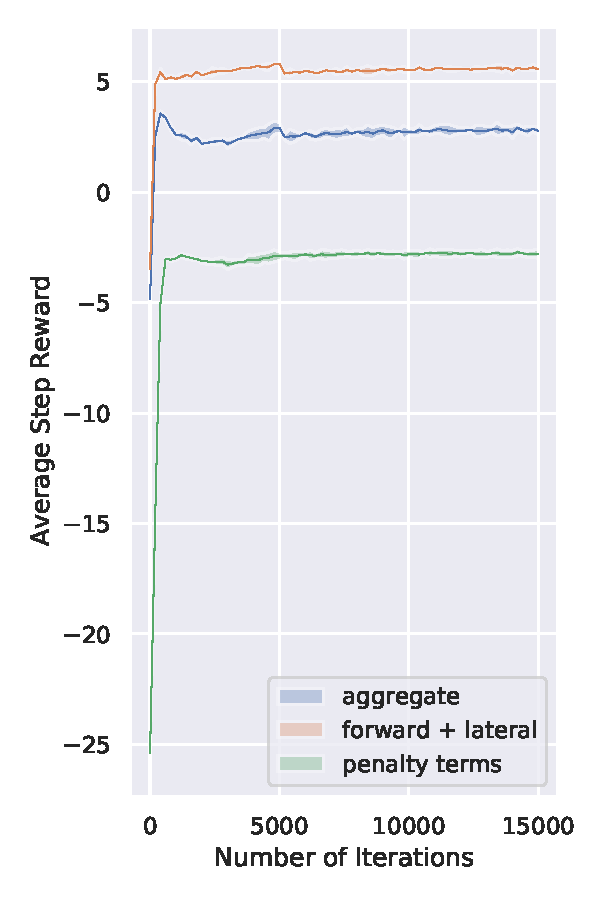
\includegraphics[width=0.75\linewidth]{figures/reward_plot.pdf}\\
  \caption{We plot the average step reward during the total $15,000$ training iterations. We show the converging trend of the reward aggregating all reward terms, forward + lateral reward, and sum of penalty terms. It also shows the necessity of applying a small multiplier to the penalty terms at the beginning of training; otherwise, the robot will only have negative experience initially and unable to learn to walk quickly.}
  \label{fig:training-reward}
\end{figure}

\section{Additional Simulation Testings}
In Figure \ref{fig:generalization_test}, we further test \algo in extreme simulated environments and show its performance in three types of environment variations: the payloads added on the base of the A1 robot, the terrain elevation variation (z-scale used in the fractual terrain generator, details in Section IV Simulation Setup of the main paper), and the friction coefficient between the robot feet and the terrain. We show the superiority of \algo across all the cases in terms of Success Rate, TTF and Reward as defined in Section \ref{sec:metrics}.



\begin{figure*}
  \centering
  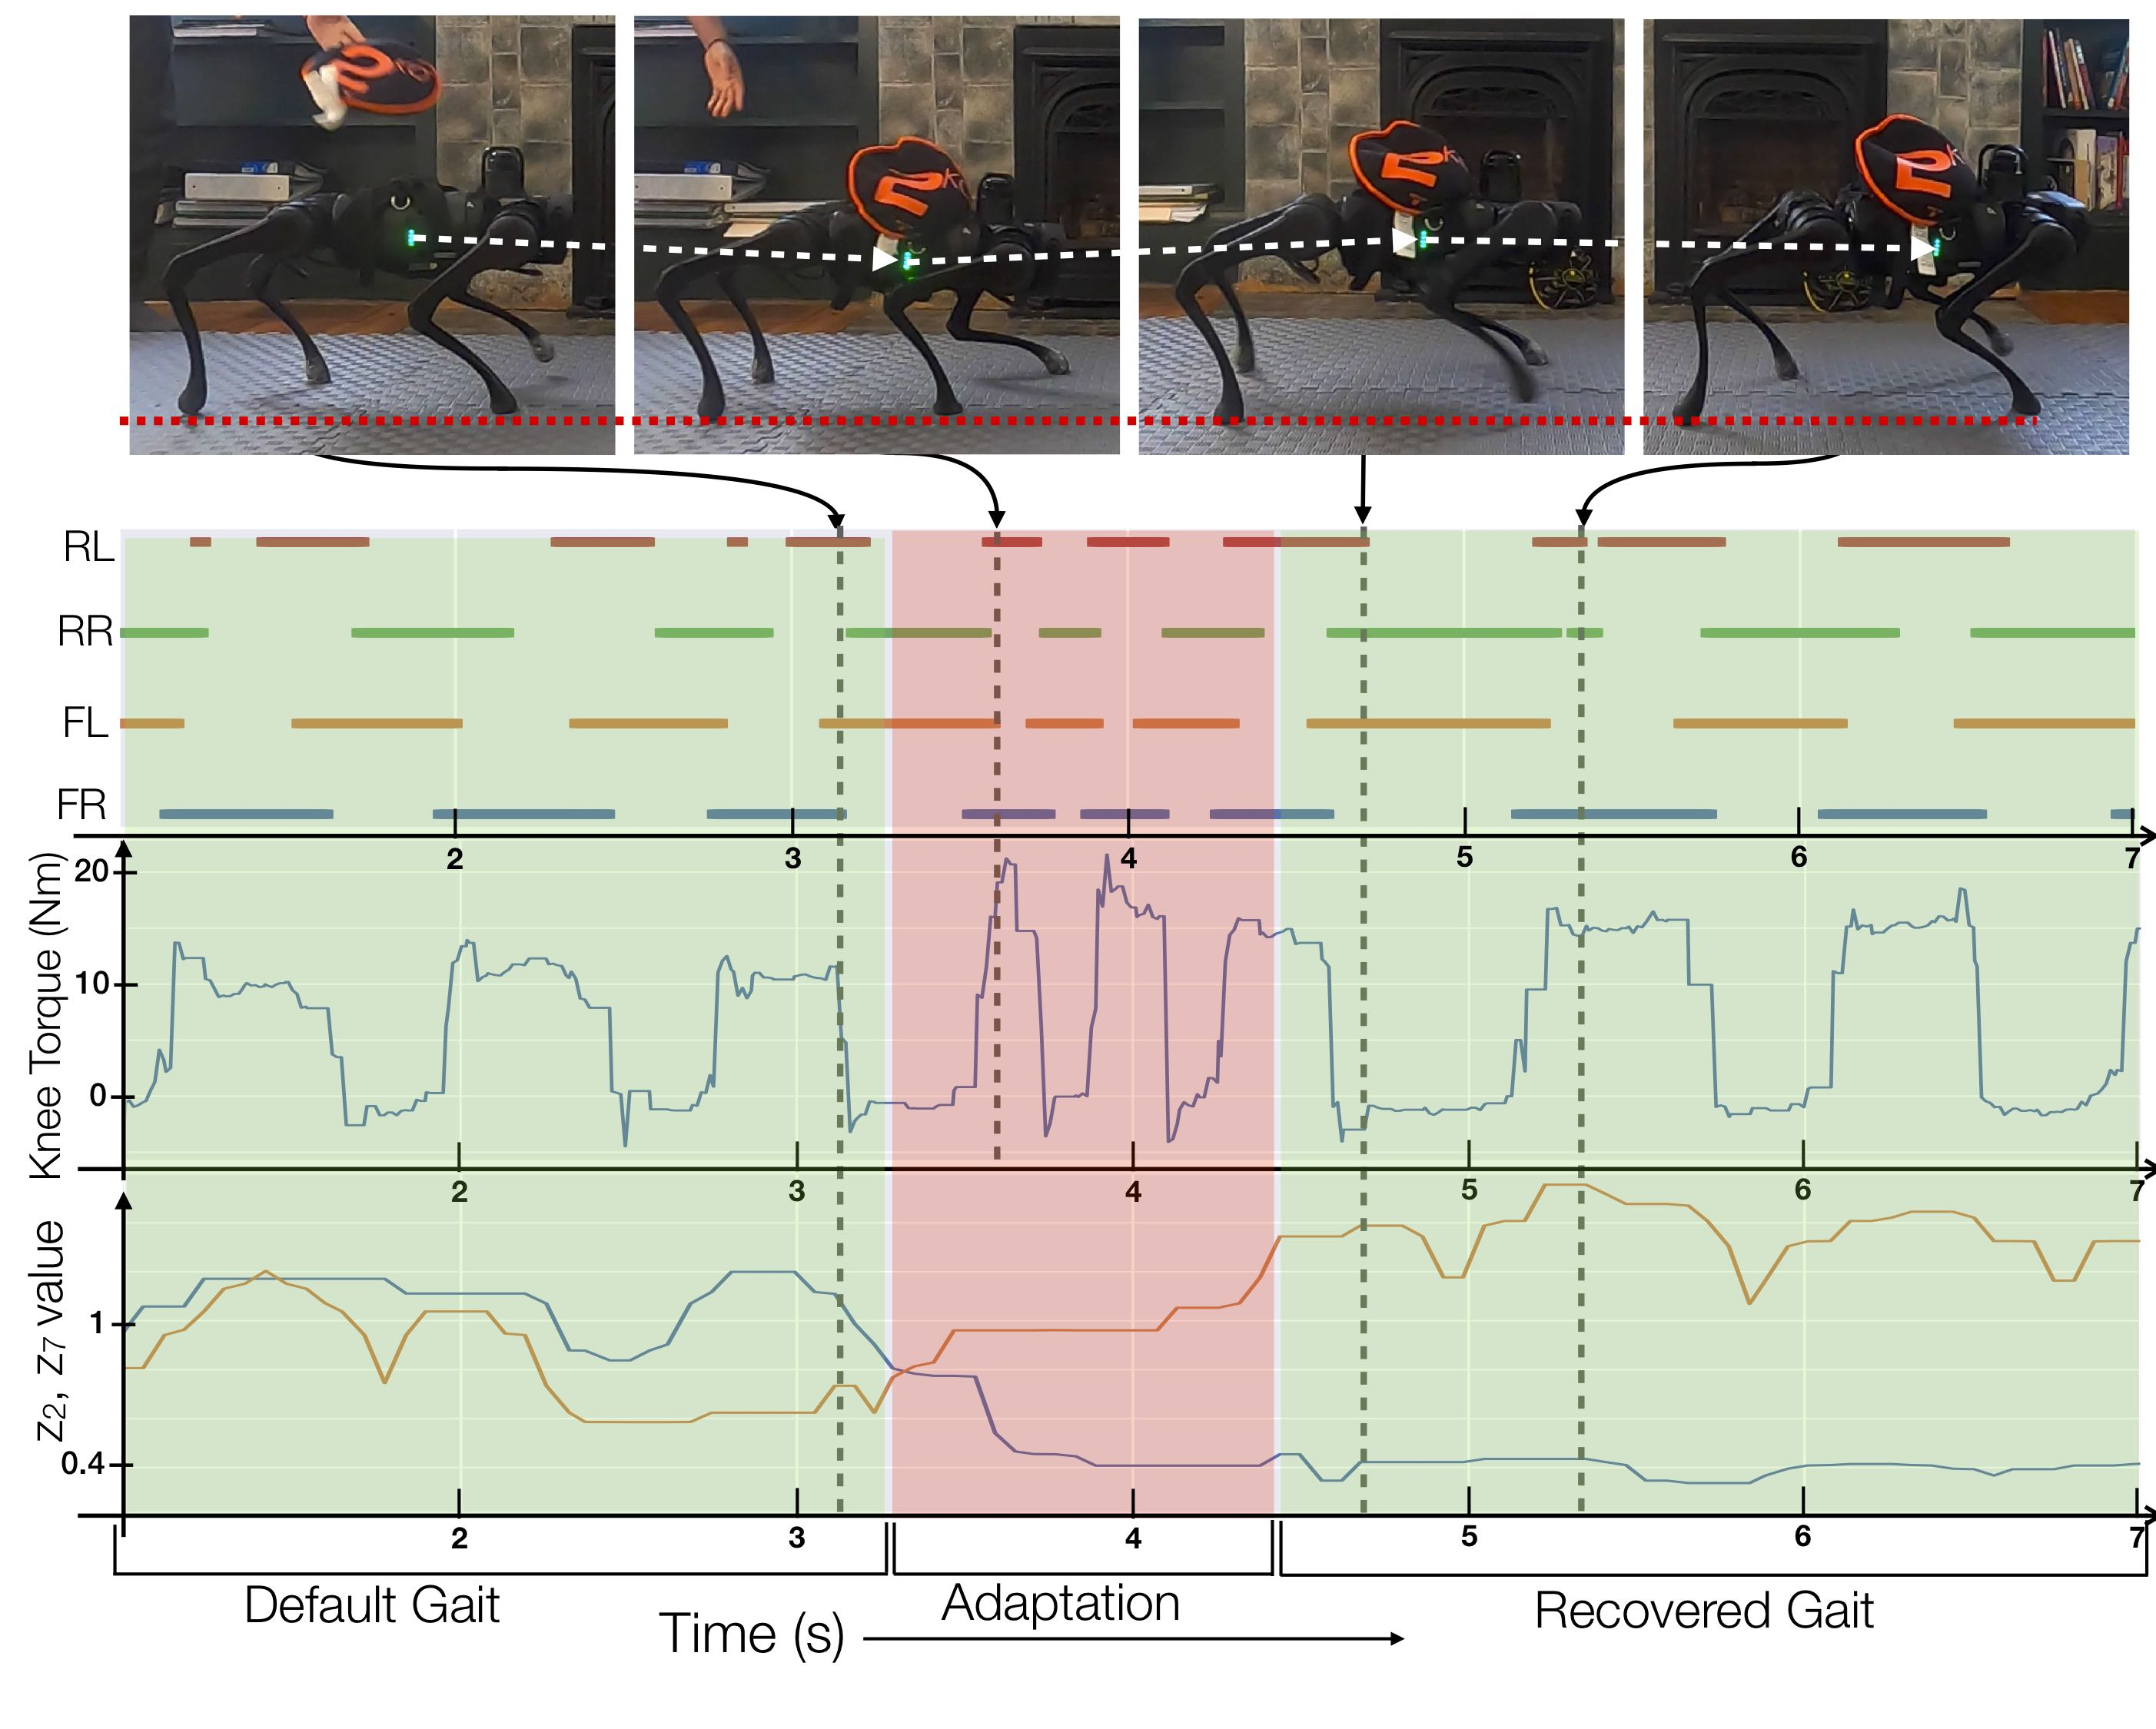
\includegraphics[width=\linewidth]{figures/mass-analysis-1.jpg}\\
  \caption{We analyze the change in behavior of \algo as we throw a payload of 5kg on the back of the robot. As a note, we have flipped the images so that that movement appears from left to right which is why the label on the sandbag appears to be 2Kg. We plot the torque profile of the knee and the gait pattern. The bottom plot shows median filtered $2^{nd}$ and $7^{th}$ components  of the extrinsics vector $\hat{z}$ predicted by the adaptation module. When the 5kg payload is thrown on the back of the robot, we see a dip in the center of mass of the robot, which the adaptation module subsequently recovers from. In the bottom plot, we see a jump in response in the plotted components of the estimated extrinsics vector, indicating that the additional payload has been detected by the adaptation module. Note that post adaptation, the recovered gait time period is roughly similar to the original, the torque magnitudes have increased and the extrinsics vector continues to capture the presence of the 5Kg payload on the back of the robot.}
  \label{fig:mass-analysis}
\end{figure*}



\begin{figure*}
  \centering
  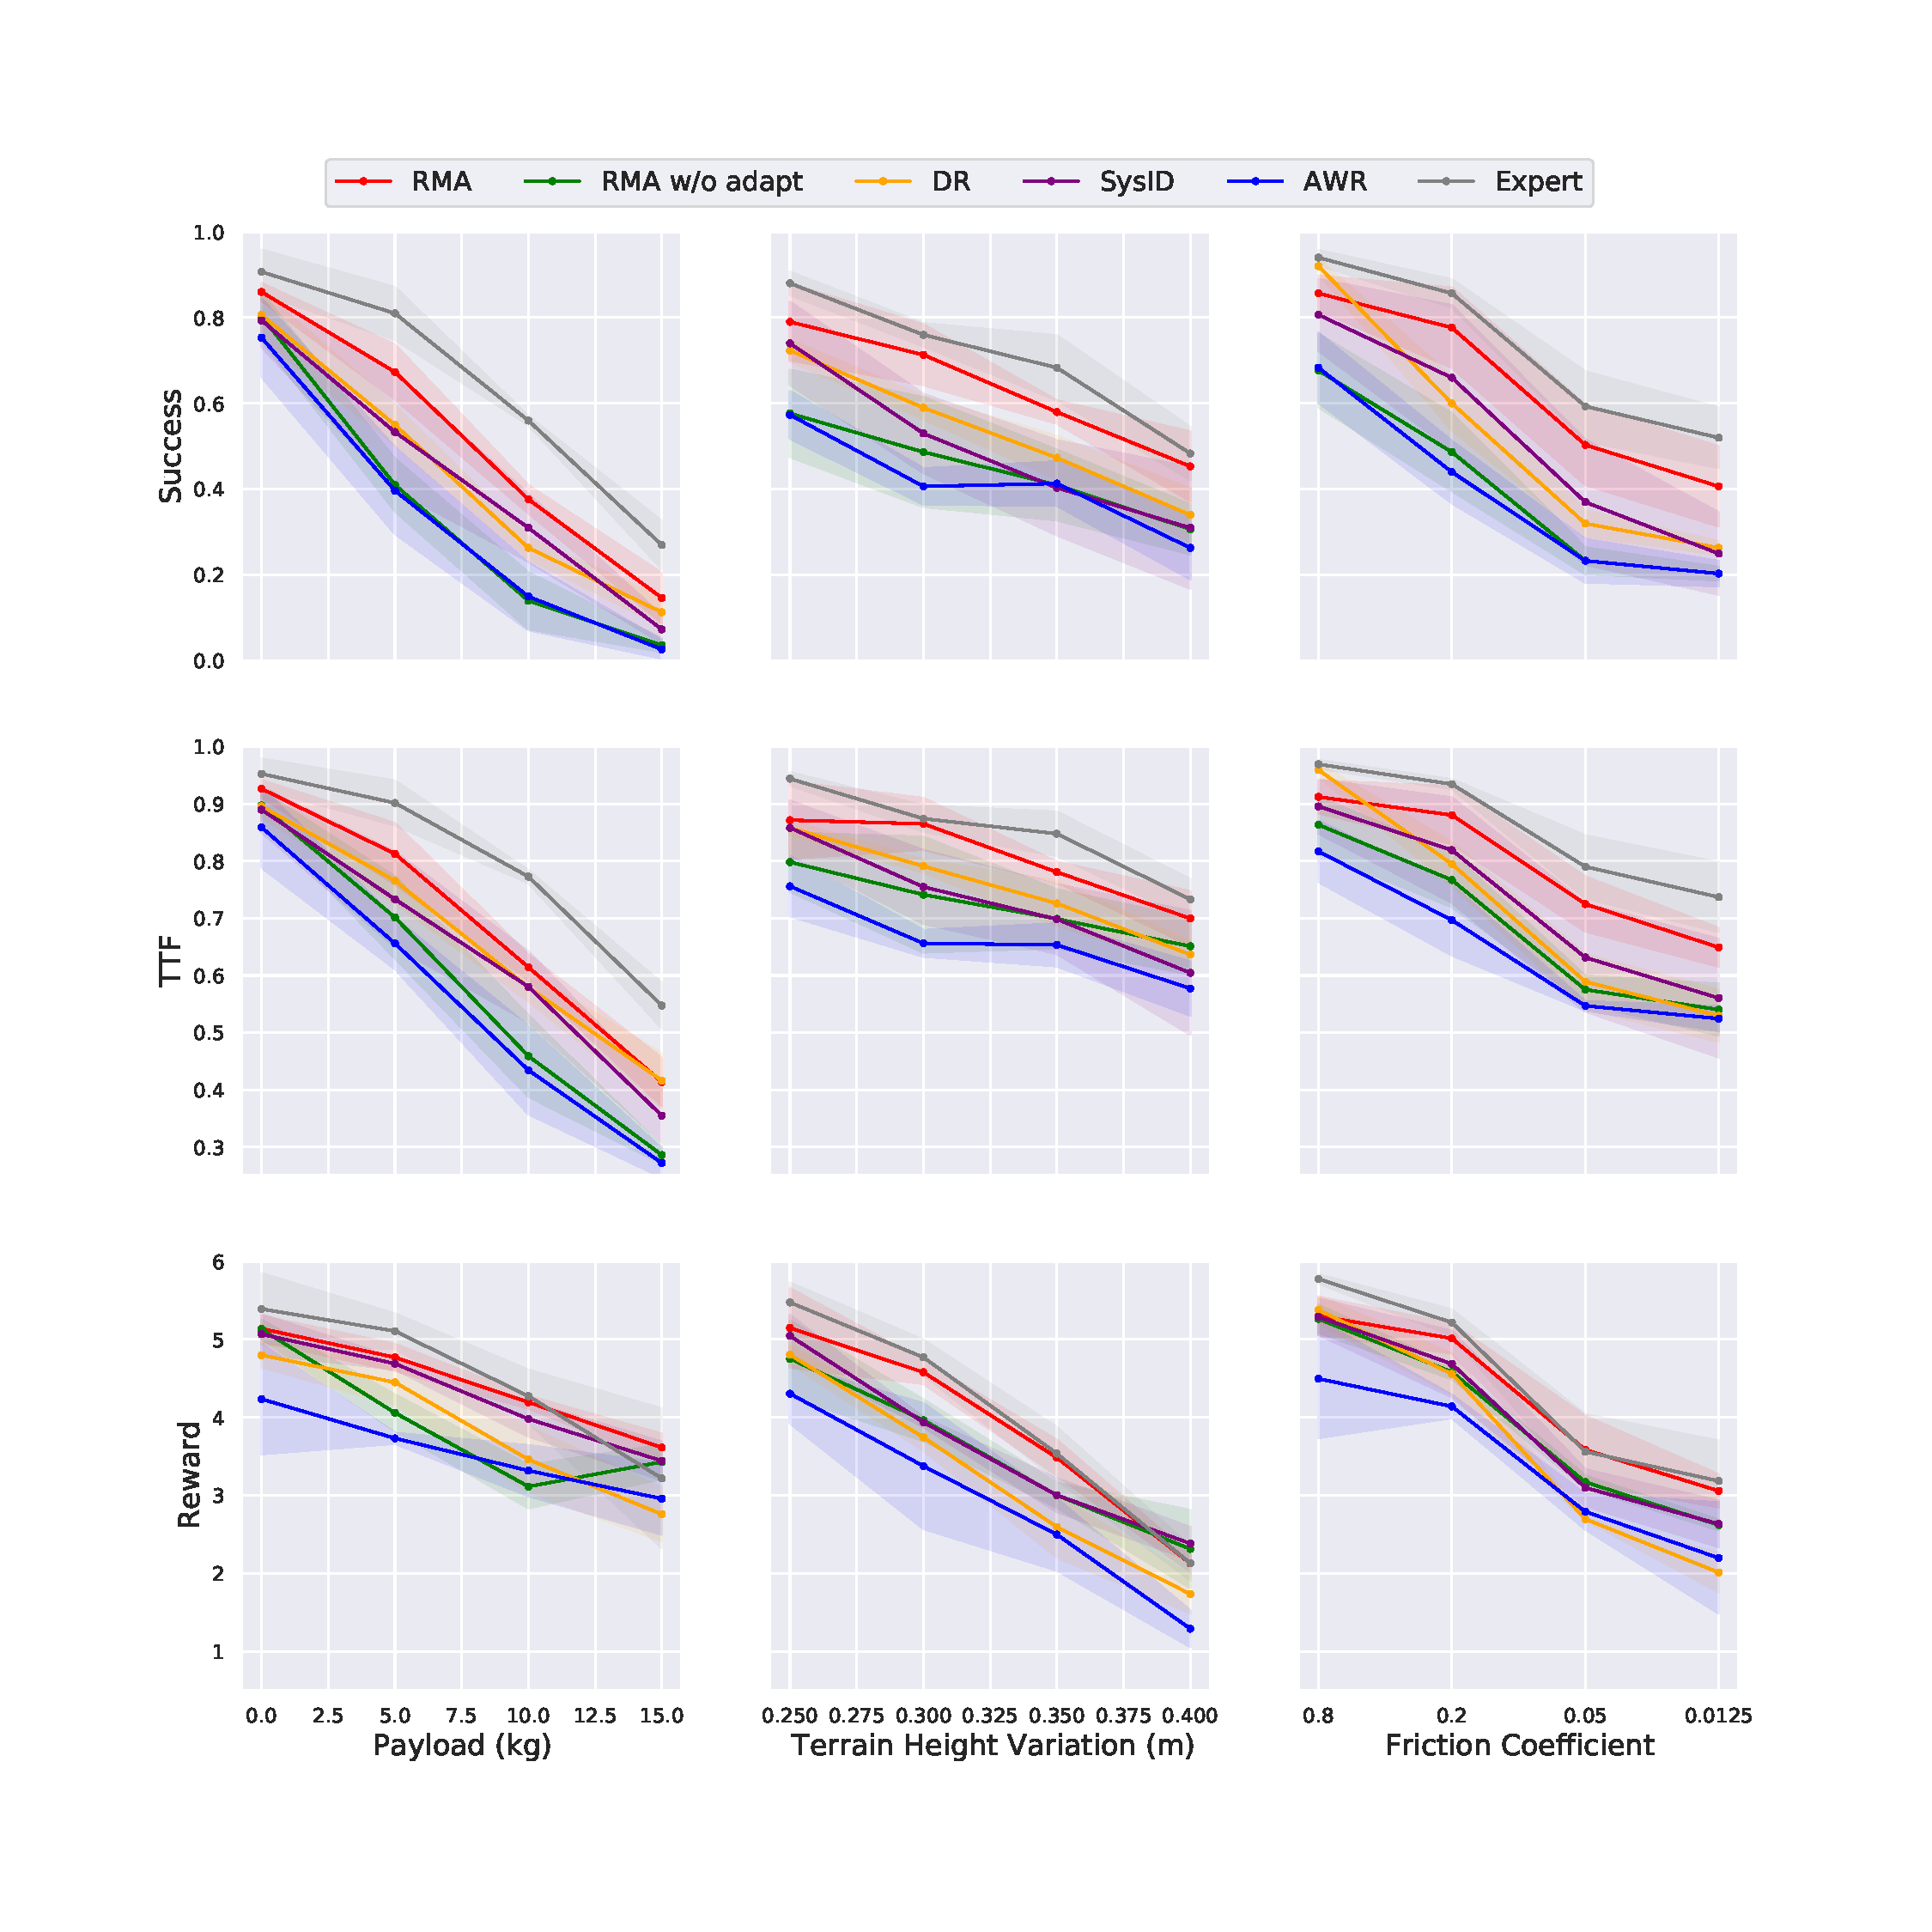
\includegraphics[height=\linewidth]{figures/generalization_test.pdf}
  \caption{\textbf{Simulation Generalization Results:} We further compare the generalization performance of our method to baseline methods in simulation. We pick three physics parameters that may vary to a large degree in the real world: the payload on robot, the terrain height variation, and the friction coefficient between the robot feet and the terrain. We set other environment parameters according to the training range in TABLE II of the main paper. Baselines and metrics are defined in Section V of the main paper and Section \ref{sec:metrics}. We report the mean and standard deviation of the performance of 3 randomly initialized policies, which is characterized by the average of 100 testing trials in given settings. Despite no testing environment samples, \algo performs the best, the closest to Expert's performance. For reference, A1 robot without additional payloads weighs $12$ kg, and is $0.35$ m tall. The static friction coefficient between rubber and concrete is $1.00$. }
  \label{fig:generalization_test}
\end{figure*}
